\documentclass[svgnames]{beamer}
\mode<presentation>
\usefonttheme{serif}
\usecolortheme{dove}
\useinnertheme{rounded}
\useoutertheme{smoothbars}
\setbeamercolor{item projected}{fg=black}
\setbeamertemplate{navigation symbols}{}

\usepackage[english]{babel}
\usepackage[latin1]{inputenc}
\usepackage{times}
\usepackage{amsthm,amssymb,amsmath,graphicx}
\usepackage{tikz}
\usetikzlibrary{arrows,automata}
%\usepackage[usenames]{color}
\usepackage{gastex}

\newcommand{\set}[1]{\{ #1 \}}
\newcommand{\fin}{\mathrm{fin}}
\newcommand{\bucf}{\mathrm{B\ddot{u}chi}(F)}
\newcommand{\parp}{\mathrm{Parity}(p)}
\newcommand{\streettrg}{\mathrm{Streett}(R,G)}
\newcommand{\infi}{\mathrm{Inf}}
\newcommand{\distk}{\mathrm{dist}_k}
\newcommand{\nextk}{\mathrm{next}_k}
\newcommand{\N}{\mathbb{N}}
\newcommand{\A}{\mathcal{A}}
\newcommand{\omegareg}{\omega\mathrm{-reg}}

\newcommand{\DB}{\mathit{DB}}
\newcommand{\DC}{\mathit{DC}}
\newcommand{\DP}{\mathit{DP}}
\newcommand{\DS}{\mathit{DS}}

\newcommand{\DFB}{\mathit{DFB}}
\newcommand{\DFC}{\mathit{DFC}}
\newcommand{\DFP}{\mathit{DFP}}
\newcommand{\DFS}{\mathit{DFS}}

\newcommand{\NB}{\mathit{NB}}
\newcommand{\NC}{\mathit{NC}}
\newcommand{\NP}{\mathit{NP}}
\newcommand{\NS}{\mathit{NS}}

\newcommand{\NFB}{\mathit{NFB}}
\newcommand{\NFC}{\mathit{NFC}}
\newcommand{\NFP}{\mathit{NFP}}
\newcommand{\NFS}{\mathit{NFS}}

\title{Finitary Languages}
\subtitle{Presentation for LATA 2011}
\author{Krishnendu Chatterjee \& \underline{Nathana\"el Fijalkow}}
\institute{IST Austria (Institute of Science and Technology, Austria)}
\date{May 30th, 2011}

\AtBeginSection[]
{
  \begin{frame}<beamer>{Outline}
    \tableofcontents[currentsection,currentsubsection]
  \end{frame}
}

\begin{document}

\begin{frame}
  \titlepage
\end{frame}

\begin{frame}{Introduction: system specification}

\only<1,2>{
\begin{itemize}
 \item non-terminating\only<1>{ (\textit{e.g} web server)};
 \item discrete time;
 \item non-deterministic.
\end{itemize}
\pause
\begin{itemize}
 \item a finite alphabet $\Sigma$ represent propositions;\\
(\textit{e.g} ``available'', ``waiting'', ``critical error'')
 \item runs are infinite words
$w = w_0 \cdot w_1 \ldots w_n \ldots \in \Sigma^\omega$;
 \item specification given as a language $L \subseteq \Sigma^\omega$.
\end{itemize}}

\only<3,4,5,6,7,8,9,10>{
\begin{center}
\begin{picture}(80,30)(0,0)
	\gasset{Nadjust=w}

	\node[Nmarks=i,iangle=-90](i)(40,0){$\emptyset$}
	\node(r1)(10,15){$R_1$}
	\node(r2)(70,15){$R_2$}
	\node(r12)(25,40){$R_1;R_2$}
	\node(r21)(55,40){$R_2;R_1$}

	\drawedge[curvedepth=6](i,r1){$R_1$}
	\drawedge[curvedepth=6](i,r2){$R_2$}
	\drawedge[curvedepth=6,dash={3 1 3 1}0](r1,i){}
	\drawedge[curvedepth=6,dash={1 1 1 1}0](r2,i){}

	\drawedge[curvedepth=12](r1,r12){$R_2$}
	\drawedge[dash={1 1 1 1}0](r12,r1){}
	\drawedge[dash={3 1 3 1}0](r12,r2){}

	\drawedge[curvedepth=-12](r2,r21){$R_1$}
	\drawedge[dash={1 1 1 1}0](r21,r2){}
	\drawedge[dash={3 1 3 1}0](r21,r1){}

	\gasset{Nadjust=n}
	\only<4,6>{\node[fillcolor=magenta,Nw=4,Nh=4](pebble)(40,0){}}
	\only<4>{\drawedge[curvedepth=6,AHLength=3,AHlength=4,
linecolor=red,linewidth=0.3](i,r1){}}
	\only<6>{\drawedge[curvedepth=6,AHLength=3,AHlength=4,
linecolor=red,linewidth=0.3](i,r2){}}
	\only<5>{\node[fillcolor=magenta,Nw=4,Nh=4](pebble)(10,15){}}
	\only<5>{\drawedge[curvedepth=6,AHLength=3,AHlength=4,
linecolor=red,linewidth=0.3](r1,i){}}
	\only<7>{\node[fillcolor=magenta,Nw=4,Nh=4](pebble)(70,15){}}
	\only<7>{\drawedge[curvedepth=-12,AHLength=3,AHlength=4,
linecolor=red,linewidth=0.3](r2,r21){}}
	\only<8,9,10>{\node[fillcolor=magenta,Nw=4,Nh=4](pebble)(55,40){}}

	\only<9>{\drawedge[AHLength=3,AHlength=4,linecolor=red,linewidth=0.7](r21,r2){}
	\put(70,0){stack strategy}}
	\only<10>{\drawedge[AHLength=3,AHlength=4,linecolor=red,linewidth=0.7](r21,r1){}
	\put(70,0){queue strategy}}
\end{picture}
\end{center}}

\only<11>{
\begin{itemize}
 \item $\omega$-regular language: safety + liveness;
 \item liveness properties: ``something good happens eventually''.
\end{itemize}}
\end{frame}

\begin{frame}{Classical liveness properties}
A first example, B\"uchi:
\begin{itemize}
 \item a given set of propositions appears infinitely often; \\
 \only<1>{(e.g ``job done'')}
\end{itemize}
\pause
\vskip2ex
A second example, Streett (fairness):
\begin{itemize}
 \item propositions are either requests $R_i$ or grants $G_i$;
 \item if $R_i$ is requested infinitely often, 
then it is serviced ($G_i$) infinitely often.
\end{itemize}
\pause
\vskip2ex
(special case: parity)
\end{frame}

\section{Motivations}

\begin{frame}{A drawback of classical $\omega$-regular specifications}
\begin{center}
\begin{picture}(80,40)(0,0)
	\gasset{Nadjust=w}

	\node[Nmarks=i,iangle=-90](i)(40,0){$\emptyset$}
	\node(r1)(10,15){$R_1$}
	\node(r2)(70,15){$R_2$}
	\node(r12)(25,40){$R_1;R_2$}
	\node(r21)(55,40){$R_2;R_1$}

	\drawedge[curvedepth=6](i,r1){$R_1$}
	\drawedge[curvedepth=6](i,r2){$R_2$}
	\drawedge[curvedepth=6,dash={3 1 3 1}0](r1,i){}
	\drawedge[curvedepth=6,dash={1 1 1 1}0](r2,i){}

	\drawedge[curvedepth=12](r1,r12){$R_2$}
	\drawedge[dash={1 1 1 1}0](r12,r1){}

	\drawedge[curvedepth=-12](r2,r21){$R_1$}
	\drawedge[dash={1 1 1 1}0](r21,r2){}

	\gasset{Nadjust=n}
	\put(70,0){stack strategy}
\end{picture}
\end{center}
\pause
\vskip2ex
Streett specification: for $i \in \set{1,2}$, if $R_i$ is requested infinitely often,
then it is serviced infinitely often.\\
\pause
\vskip2ex
Satisfied, but the ``service time'' may grow unbounded!
\end{frame}

\begin{frame}{A stronger formulation of liveness: finitary liveness~\cite{AH94}}
Intuitively: there exists an \textbf<2>{unknown}, fixed bound $b$ 
such that good things happen within $b$ transitions.
\pause
\only<2>{\vskip1ex\textbf{unknown}: retain independence from granularity.}
\pause
\vskip2ex
It can be expressed as a finitary operator on languages:
$$\fin(L) = \bigcup \set{M \mid M \textrm{ closed and } \omega \textrm{-regular}, M \subseteq L}$$
\pause
\begin{itemize}
 \item closed: involves Cantor topology;
 \item $\omega$-regular: involves $\omega$-regularity;
 \item restriction operator: $\fin(L) \subseteq L$.
\end{itemize}
\end{frame}

\begin{frame}{Back to the example}
\begin{center}
\begin{picture}(80,40)(0,0)
	\gasset{Nadjust=w}

	\node[Nmarks=i,iangle=-90](i)(40,0){$\emptyset$}
	\node(r1)(10,15){$R_1$}
	\node(r2)(70,15){$R_2$}
	\node(r12)(25,40){$R_1;R_2$}
	\node(r21)(55,40){$R_2;R_1$}

	\drawedge[curvedepth=6](i,r1){$R_1$}
	\drawedge[curvedepth=6](i,r2){$R_2$}
	\drawedge[curvedepth=6,dash={3 1 3 1}0](r1,i){}
	\drawedge[curvedepth=6,dash={1 1 1 1}0](r2,i){}

	\drawedge[curvedepth=12](r1,r12){$R_2$}

	\drawedge[curvedepth=-12](r2,r21){$R_1$}

	\gasset{Nadjust=n}
\only<1,2>{\put(70,0){stack strategy}
	\drawedge[dash={1 1 1 1}0](r12,r1){}
	\drawedge[dash={1 1 1 1}0](r21,r2){}}

\only<3,4>{\put(70,0){queue strategy}
	\drawedge[dash={3 1 3 1}0](r12,r2){}
	\drawedge[dash={3 1 3 1}0](r21,r1){}
}
\only<2>{\put(21,20){\huge{{\color{red}{Not satisfied!}}}}}
\only<4>{\put(27,20){\huge{{\color{red}{Satisfied!}}}}}	
\end{picture}
\end{center}
\vskip2ex
Finitary Streett specification: there exists a bound $b$, 
such that \textit{in the limit},
for $i \in \set{1,2}$, if $R_i$ is requested,
then it is serviced within $b$ transitions.
\end{frame}

\section{Characterizations}

\begin{frame}{Describing classical finitary objectives: B\"uchi}
Let $F \subseteq \Sigma$,
$$\bucf = \set{ w \mid \infi(w) \cap F \not= \emptyset}$$
\only<1>{\vskip1ex $\infi(w)$ is the set of propositions that appear infinitely often in $w$.}
\pause
$$\nextk (w,F) = \inf \set{k'-k \mid k' \geq k, w_{k'} \in F}$$
\pause
\only<3>
{
$$w = v_0 \ldots v_k \underbrace{v_{k+1} \ldots v_{k'-1}}_{\notin F} \underbrace{v_{k'}}_{\in F}$$
waiting time from the $k$\textsuperscript{th} position.
}
\pause
\begin{lemma}
$$\fin(\bucf) = \set{w \mid \limsup_k \nextk (w,F) < \infty}$$
\end{lemma}
\end{frame}

\begin{frame}{Topological classification in Borel hierarchy}

%\begin{theorem}
%$\bucf$ is $\Pi_2$-complete.
%\end{theorem}
%\pause

\begin{theorem}
$\fin(\bucf)$, $\fin(\parp)$ and $\fin(\streettrg)$ are $\Sigma_2$-complete.
\end{theorem}
\end{frame}

\begin{frame}{Automata-theoretic expressive power}

We consider automata over infinite words, 
whose acceptance conditions are finitary B\"uchi, finitary parity or
finitary Streett.\\
\pause
A finitary B\"uchi automaton is $\A = (Q, \Sigma, Q_0, \delta, \fin\bucf)$.
\pause
$$\left \{ \begin{array}{c} D \\ N \end{array} \right \} \cdot
\left \{ \begin{array}{c} \varepsilon\ (classical) \\ F (finitary) 
\end{array} \right \} \cdot
\left \{ \begin{array}{c} B\ (B\ddot{u}chi) \\ P\ (parity) \\ S\ (Streett) 
\end{array} \right \}$$
\end{frame}

\begin{frame}{}
\begin{figure}
\centering
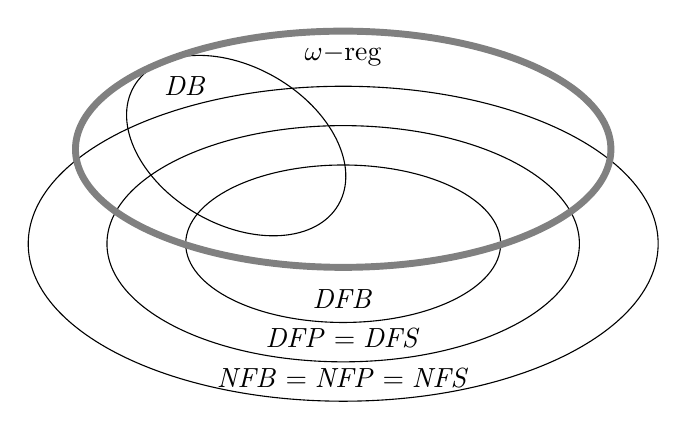
\begin{tikzpicture}
   \draw[rotate=90] (0,0) ellipse (1cm and 2cm);
   \draw[rotate=90] (0,0) ellipse (1.5cm and 3cm);
   \draw[rotate=90] (0,0) ellipse (2cm and 4cm);

   \draw[rotate=60] (.4,1.8) ellipse (1cm and 1.5cm);

   \draw[rotate=90,color=gray,line width=2.5pt] (1.2,0) ellipse (1.5cm and 3.4cm);
   \draw (0,-0.7) node {$\DFB$}; 
   \draw (0,-1.2) node {$\DFP = \DFS$};
   \draw (0,-1.7) node {$\NFB = \NFP = \NFS$};  
   \draw (-2,2) node {$\DB$};
   \draw (0,2.4) node {$\omegareg$};  
\end{tikzpicture}
\caption{Expressive power classification}\label{fig_automata}
\end{figure}
\end{frame}

\section{Expressions}

\begin{frame}{Regular and $\omega$-regular expressions}
Regular expressions defines regular languages over finite words:
$$L := \emptyset \mid \varepsilon \mid \sigma 
\mid \underbrace{L \cdot L}_{\textrm{concatenation}}
\mid \underbrace{L^*}_{\textrm{star}} 
\mid \underbrace{L + L}_{\textrm{union}}; 
\quad \sigma \in \Sigma$$

$\omega$-regular languages are finite union of $L_1 \cdot L_2^\omega$,
where $L_1$ and $L_2$ are regular languages over finite words.
\end{frame}

\begin{frame}{The bound operator $B$~\cite{BC06}}
$$L^\omega = \set{u_0 \cdot u_1 \cdot \ldots \cdot u_k \ldots \mid u_0, u_1, \ldots, 
u_k,\ldots \in L}$$
\pause
\texttt{Example:} $(a^* \cdot b)^\omega$ expresses ``infinitely many $b$'s''.
\pause

\texttt{Example:} $(a^B \cdot b)^\omega$ expresses 
``infinitely many $b$'s with an upper bound on the length of $a$'s blocks''.
%(complete definitions for $B$ requires more work)
\end{frame}

\begin{frame}{Star-free $\omega B$-regular expressions}

$B$-regular languages are described by the grammar:
$$M := \emptyset \mid \varepsilon \mid \sigma \mid M \cdot M \mid 
M^* \mid M^B \mid M + M; \quad \sigma \in \Sigma$$

\only<1,2>{
$\omega B$-regular languages are finite union of $L \cdot M^\omega$, where 
\begin{itemize}
 \item $L$ is a regular language over finite words;
 \item $M$ is a $B$-regular language over infinite words.
\end{itemize}}

\pause
\textbf{Star-free} $\omega B$-regular languages are finite union of 
$L \cdot M^\omega$, 
where 
\begin{itemize}
 \item $L$ is a regular language over finite words;
 \item $M$ is a \textbf{star-free} $B$-regular language over infinite words.
\end{itemize}
``no star operator under the $\omega$-operator''.

\end{frame}

\begin{frame}{Equivalence}
\begin{theorem}
$\NFB$ (non-deterministic finitary B\"uchi automata) has exactly 
the same expressive power as star-free $\omega B$-regular expressions.
\end{theorem}
\end{frame}

\begin{frame}{Examples}

\texttt{First example:} $c^* \cdot (a^B \cdot b)^\omega$ 
is a star-free $\omega B$-regular expression,
\pause
it expresses ``a finite number of $c$'s followed by 
an infinite word over alphabet $\set{a,b}$,
with infinitely many $b$'s and an upper bound on the length of $a$'s blocks''.
\pause

\texttt{Second example:} $(a^B \cdot b \cdot (a^* \cdot b)^*)^\omega$ 
is \textbf{not} a star-free $\omega B$-regular expression,
\pause
it expresses ``words of the form $a^{n_0} \cdot b \cdot a^{n_1} \cdot b \ldots $
such that $\liminf_i n_i < \infty$''.

\end{frame}

\begin{frame}{Conclusion}
\begin{itemize}
 \item finitary objectives is a refinment for specification purposes;
 \item for $\omega$-regular languages, topological, logical and automata-theoretic 
studies are well-known;
 \item for finitary languages, all were missing; we established:
 \begin{itemize}
  \item topological classification;
  \item automata-theoretic characterization, 
 comparison to $\omega$-regular languages,
 closure properties;
  \item characterization using by $\omega B$-regular expressions. 
 \end{itemize} 
\end{itemize}
\pause
Future work:
\begin{itemize}
 \item games (work in progress);
 \item a finitary logic, Myhill-Nerode equivalence relations, \ldots
\end{itemize}
\end{frame}

\begin{frame}{Bibliography}
\bibliography{bib}
\bibliographystyle{alpha}
\end{frame}

\begin{frame}{The end}
\begin{center}
Thank you for your attention!
\end{center}
\end{frame}

\end{document}